\begin{figure}[H]
\centering
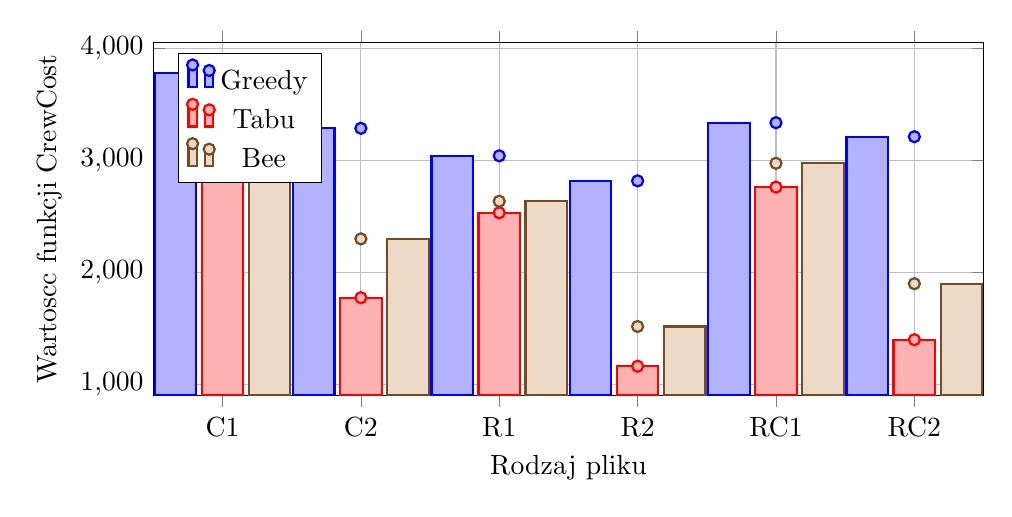
\begin{tikzpicture}
\begin{axis}[
xlabel = {Rodzaj pliku},
ylabel = {Wartoscc funkcji CrewCost},
legend pos = north west,
grid = both,
width=1\linewidth,
height=0.5\linewidth,
ybar,
bar width=15pt,
symbolic x coords={C1,C2,R1,R2,RC1,RC2,},
xtick=data
]
\addplot + [mark = *, thick] coordinates
    {
(C1,3777.777777777778)(C2,3287.5)(R1,3041.6666666666665)(R2,2818.181818181818)(RC1,3337.5)(RC2,3212.5)};
\addlegendentry
{Greedy}
\addplot + [mark = *, thick] coordinates
    {
(C1,3788.8888888888887)(C2,1775.0)(R1,2533.3333333333335)(R2,1163.6363636363637)(RC1,2762.5)(RC2,1400.0)};
\addlegendentry
{Tabu}
\addplot + [mark = *, thick] coordinates
    {
(C1,3644.4444444444443)(C2,2300.0)(R1,2636.3636363636365)(R2,1518.1818181818182)(RC1,2975.0)(RC2,1900.0)};
\addlegendentry
{Bee}
\end{axis}
\end{tikzpicture}
\caption
{Porownanie srednich wartosci CrewCost algorytmow dla kazdego rodzaju pliku}
\label{fig:mean_CrewCost_comparision}
\end{figure}
